\section{Introduzione}
    \begin{center}
        \Large\color{red}!!!DISCLAIMER!!!
    \end{center}
    Questo corso si basa fortemente sullo studio del libro \textit{Sistemi Operativi: Concetti ed Esempi} di \textit{Abraham Silberschatz}. I seguenti appunti fungono dunque da guida e riassunto di quanto studiato sul libro, ma non hanno una funzione sostitutiva. I riferimenti a pagine e capitoli del libro sono riguardanti la decima edizione Italiana.
    
    L'obiettivo di questo corso, dal punto di vista teorico, è capire con un certo livello di precisione e dettaglio cosa sia un sistema operativo, le motivazioni dietro lo stesso e come funzioni. Dal punto di vista pratico sarà scrivere un programma che invoca correttamente delle \texttt{syscall} (system calls). Questo percorso ha inizio con questa prima parte, che comprende delle definizioni di base di sistema operativo, dei cenni storici e uno studio della struttura di un sistema operativo.
    
\section{Cosa è un Sistema Operativo}
    Un Sistema Operativo è innanzitutto un \textbf{programma}, nonostante abbia struttura e funzioni piuttosto diverse da quelle dei programmi con cui siamo abituati a interagire.
    
    Per capire la funzione di un SO e in che modo è diverso da tutti gli altri programmi, ci conviene posizionarlo all'interno di un contesto software e hardware:
    
    \begin{figure}[h]
        \centering
        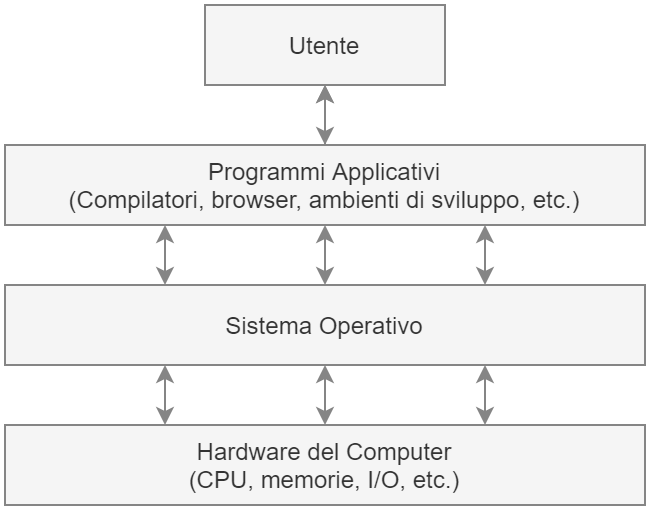
\includegraphics[width=0.6\textwidth]{img/img1.png}
        \caption{Componenti di un sistema elaborativo.}
        \label{fig:img1}
    \end{figure}
    
    Facciamo dunque una suddivisione dell'intero sistema elaborativo in quattro componenti, e in particolare vediamo che l'\textbf{hardware} fornisce al sistema le risorse di memorizzazione ed elaborative fondamentali, mentre i \textbf{programmi applicativi} definiscono il modo in cui queste risorse vengono usate nella risoluzione di problemi computazionali degli \textbf{utenti}, i quali si interfacciano con i suddetti programmi. 
    
    In tutto ciò, il ruolo del \textbf{sistema operativo} è quello di offrire gli strumenti per impiegare in modo corretto le risorse offerte. Il suo ruolo, per fare un'analogia politica, è simile a quello di un \textit{governo}, che non svolge funzioni effettivamente utili, ma fornisce un ambiente nel quale altri enti/programmi possono lavorare in modo utile.
    
    Per meglio capire il ruolo del sistema operativo, e per avere un altro punto di vista, lo esploriamo da due punti di vista: quello dell'utente e quello del sistema.
    
    \subsection{Punto di vista dell'utente}
        Dal punto di vista di un utente che usa un determinato dispositivo, la cosa più importante è la \textbf{facilità d'uso}. I sistemi operativi odierni sono generalmente progettati per l'utilizzo da parte di un singolo utente, con grande attenzione alla suddetta facilità d'uso, qualche accortezza riguardante le prestazioni, ma nessuna all'\textbf{utilizzo delle risorse}, a come cioè sono condivise le risorse hardware e software.
        
        Un altro punto da prendere in considerazione è la varietà dei dispositivi utilizzati dai vari utenti, che possono andare dai più classici personal computer dotati di schermo, tastiera e mouse, agli smartphone, dotati di touch screen e assistenti vocali, a dispositivi \textbf{embedded} presenti in elettrodomestici e simili, che possono interfacciarsi con l'utente in maniera molto minimale, tramite magari una tastiera numerica, qualche tasto e dei led per indicarne lo stato.
        
    \subsection{Punto di vista del sistema}
        Dal punto di vista del calcolatore, il sistema operativo è il programma più strettamente correlato al suo hardware. In tale contesto è possibile considerare un sistema operativo come un \textbf{assegnatore di risorse}.
        
        Un altro modo per vedere il sistema operativo è come programma di controllo che gestisce l'esecuzione di programmi utenti in modo da impedire eventuali errori o che il calcolatore sia usato in modo scorretto, e che si occupa del controllo dei dispositivi I/O, con un'enfasi non primaria sull'ottimizzazione delle risorse.
        
    \subsection{Definizione di Sistema Operativo}
        A questo punto abbiamo capito che non è semplicissimo dare una definizione precisa di sistema operativo. Esso definisce diversi ruoli e funzionalità e ciò può variare in base alla natura del sistema hardware, ai target users e tanti altri parametri.
        
        Nonostante tutto ciò, per i nostri scopi il sistema operativo include il kernel (nucleo) sempre in esecuzione, i framework middleware che facilitano lo sviluppo di applicazioni e forniscono altre funzionalità e i programmi di sistema che contribuiscono alla gestione dello stesso mentre è in esecuzione.
        
\newpage
\section{Organizzazione di un sistema elaborativo}
    \begin{figure}[h]
        \centering
        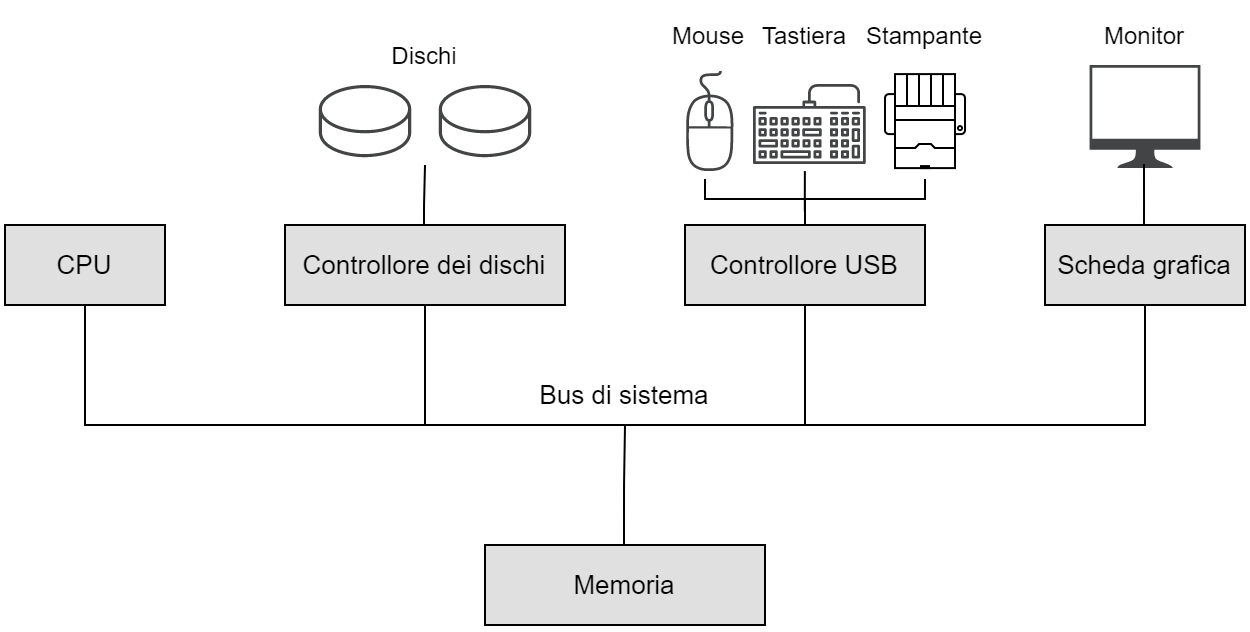
\includegraphics[width=0.9\textwidth]{img/img2.png}
        \caption{Un tipico sistema elaborativo}
        \label{fig:img2}
    \end{figure}
    
    Un moderno computer ha una o più (ma spesso più) CPU e un certo numero di controllori di dispositivi connessi attraverso un canale di comunicazione comune detto \textit{bus}, che permette l'accesso alla memoria condivisa del sistema.
    
    Il sistema operativo entra in gioco con i \textbf{driver del dispositivo}. Esso dispone di un driver per ogni controllore di dispositivo, che gestisce le specificità del controllore e funge da interfaccia con il resto del sistema.
    
    Andremo ora a descrivere in che modo il sistema operativo può garantire l'accesso concorrente e parallelo ai controllori, concentrandoci su tre aspetti chiave: interrupt, struttura della memoria e struttura I/O.
    
    \subsection{Interrupt}
        Un controllore che esegue un'operazione dovrà informare il sistema operativo, tramite il driver, di averla conclusa così da far eseguire le operazioni appropriate, come dare un output, restituire dati o semplicemente restituire il controllo. Come fa il controllore a comunicare al driver del dispositivo che ha terminato la sua operazione? Tramite un'\textbf{interruzione}, o \textit{interrupt}.
        
        
        \paragraph{Come una interrupt viene inviata.} Le \textbf{interruzioni} possono essere usate per vari scopi e costituiscono una componente chiave nell'interazione fra i sistemi operativi e l'hardware. Quest'ultimo può generare un'interruzione in qualsiasi momento inviando un segnale alla CPU, solitamente tramite il bus di sistema (un sistema di elaborazione può avere svariati bus, ma quello di sistema è il principale percorso di comunicazione fra i componenti fondamentali).
        
        \paragraph{Come una interrupt viene gestita.} Quando riceve una \textit{interrupt}, la CPU interrompe immediatamente l'elaborazione corrente, salva il suo stato e trasferisce l'esecuzione a una locazione fissa della memoria. Di solito questa locazione contiene l'indirizzo iniziale della procedura di servizio dell'interruzione. Una volta completata l'operazione, la CPU riprende qualsiasi operazione stesse eseguendo precedentemente.
        
        \paragraph{Come realizzare le interrupt.} Le interrupt sono un'operazione molto sensibile. Esse devono essere molto veloci, in quanto potrebbero avvenirne anche centinaia di volte al secondo. Un modo per realizzare ciò è creare una tabella di puntatori alle specifiche procedure richieste dalla interrupt, e memorizzarla in indirizzi di memoria bassi (per esempio i primi 100), così da potervi accedere direttamente senza operazioni intermedie. Molte funzioni riguardanti le interruzioni sono abbastanza comuni, basti pensare che sistemi operativi molto diversi come Windows e UNIX hanno lo stesso meccanismo di gestione delle interruzioni.
        
        \paragraph{Implementazione.}
            Il meccanismo alla base dell'implementazione della gestione delle interruzioni è piuttosto semplice. L'hardware disponde di un filo chiamato \textit{interrupt-request line} che la CPU controlla dopo l'esecuzione di ogni istruzione. Quando la CPU rileva un'interruzione la gestisce leggendone il numero di interruzione e saltando alla routine associata. Viene eseguito il salvataggio di informazioni che verranno modificate, l'elaborazione e il \texttt{return\textunderscore from\textunderscore interrupt} che ci riporta allo stato precedente.
            
            In altre parole il controllore del dispositivo \textit{solleva} un'interruzione, la CPU la \textit{intercetta} e la \textit{invia} al gestore delle interruzioni che a sua volta soddisfa la richiesta.
            
            Il meccanismo appena descritto è semplice ed efficace, ma in un sistema operativo moderno sono necessarie operazioni più sofisticate, come:
            \begin{enumerate}
                \item Possibilità di posticipare la gestione degli interrupt durante un'operazione critica.
                \item Metodo efficiente per inviare l'interruzione al gestore appropriato per un dato dispositivo.
                \item Interruzioni multilivello, con vari gradi di priorità.
            \end{enumerate}
            
            In un'architettura moderna queste tre funzioni sono fornite dalla CPU e dall'hardware del controllore delle interruzioni.
            
            La maggior parte delle CPU ha due linee di richiesta delle interruzioni: una viene detta \textbf{non mascherabile} (\textit{nonmaskable interrupt}) ed è riservata a eventi come errori irreversibili i memoria, mentre la seconda è \textbf{mascherabile} (\textit{maskable interrupt}), ovvero può essere disattivata dalla CPU prima dell'esecuzione di istruzioni critiche. L'interruzione mascherabile è quella usata dai controllori di dispositivi per richiedere un servizio.
            
    \newpage
    \subsection{Struttura della memoria}
        La memoria può essere ordinata in base a una gerarchia, che traccia un compromesso fra la capacità di archiviazione e il tempo di accesso; meno dati possono essere conservati sulla memoria, più velocemente è possibile accedervi. Infatti, per fare alcuni esempi, abbiamo in ordine dal meno capiente ma più veloce al più capiente ma meno veloce: registri, cache, dischi magnetici, etc...
        
        Un'altra distinzione importante è fra le memorie volatili e non volatili. Le prime perdono i dati immagazzinati quando viene tolta la fonte di energia che le alimenta, mentre le non volatili mantengono permanentemente i loro dati.
        
        In questo corso faremo riferimento alla memoria volatile come semplicemente \textbf{memoria}, mentre quella non volatile con l'acronimo \textbf{NVS}. Eventuali dispositivi specifici verranno specificati.
        
    \subsection{Struttura di I/O}
        Una cospicua parte di codice di un sistema operativo è dedicata alla gestione di I/O. Tutta via l'I/O guidato dalle interruzioni precedentemente descritto risulta poco efficace in alcuni casi, basti pensare al trasferimento di massicce quantità di dati da e verso NVS.
        
        La soluzione è l'\textbf{accesso diretto alla memoria} (\textbf{DMA}, o \textit{direct memory access}). Una volta impostati i buffer, i puntatori e i contatori necessari al dispositivo di I/O, il controllore spedisce un intero blocco dati dal proprio buffer alla memoria centrale, senza intervento della CPU, richiedendo così una interrupt per ogni blocco dati anziché per ogni byte.
    
\section{Architettura degli elaboratori}
    \subsection{Sistemi monoprocessore e multiprocessore}
            Per sistema monoprocessore intendiamo un qualsiasi sistema con un solo core. Un sistema potrebbe avere microprocessori specializzati, come per esempio un microprocessore nella tastiera che individua e comunica la pressione esercitata sui tasti, ma questo non rende un sistema multiprocessore.
            
            Pochissimi computer moderni sono monoprocessore. Nel panorama moderno i sistemi multiprocessore sono l'alternativa più diffusa. Un tale sistema dispone di due o più processori, ognuno dotato di una singola unità di calcolo. Il vantaggio è di ottenere una maggiore capacità elaborativa (\textit{throughput}). Tuttavia aumentando di \textit{N} volte il numero di core, non aumenta di \textit{N} volte la capacità di elaborazione, siccome è necessario del lavoro supplementare (\textit{overhead}) per garantire che tutti i componenti funzionino correttamente.
            
            La modalità più diffusa di elaborazione parallela è la \textbf{SMP}, o \textbf{multielaborazione simmetrica}, in cui ogni processore, alla pari degli altri, è abilitato all'esecuzione di tutte le funzioni del sistema.
            
            \begin{figure}[h]
                \centering
                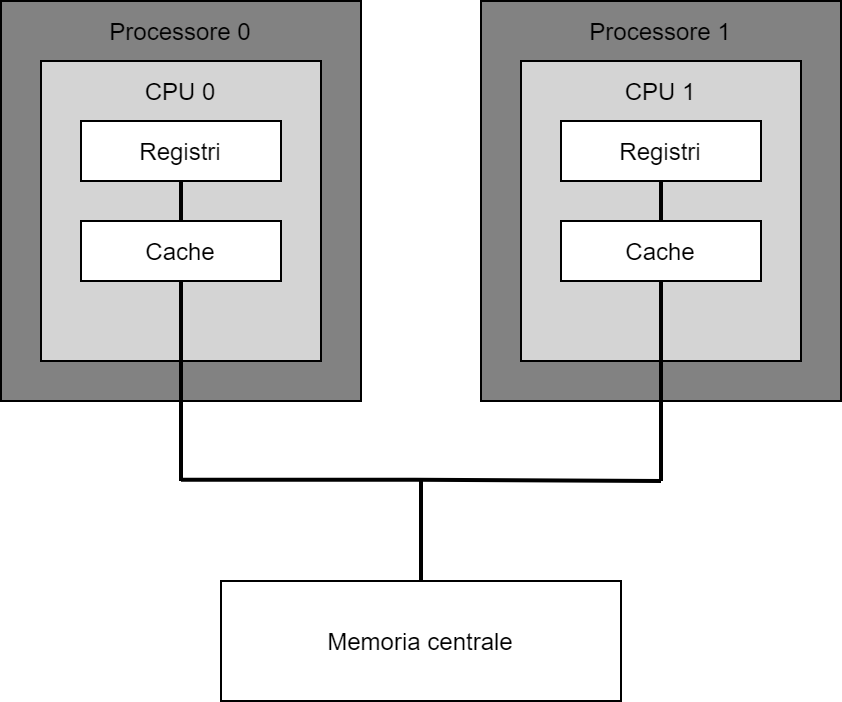
\includegraphics[width=0.85\textwidth]{img/img3.png}
                \caption{Architettura di multielaborazione simmetrica}
                \label{fig:img3}
            \end{figure}
            
            \newpage
            Nonostante ogni core abbia un suo set di registri e una cache privata, condividono la memoria fisica sullo stesso bus di sistema.
            
            Il vantaggio di questo tipo di sistema è che per \textit{N} processori, \textit{N} processi possono essere eseguiti contemporaneamente senza un rilevante calo delle prestazioni. Tuttavia potrebbe capitare che un processore è in sovraccarico, mentre l'altro è totalmente inattivo. Questo potrebbe essere risolto permettendo ai processori di condividere alcune strutture dati, ma come vedremo in futuro, ciò va implementato con molta attenzione.
            
            La definizione di \textbf{multiproccessore} si è evoluta col tempo e oggi include sistemi in cui più CPU risiedono in un singolo chip. Questo è conveniente da un punto di vista computazionale in quanto lo scambio di dati all'interno di uno stesso chip è più veloce di uno scambio fra chip diversi. Inoltre un chip richiede una potenza minore per essere alimentato, cosa molto utile nei sistemi a batteria come smartphone e laptop.
            
            Questo ultimo stile di architettura è il più utilizzato e oltre a considerazioni su condivisione della memoria, delle risorse e accessi, al sistema operativo queste CPU multicore appaiono come \textit{N} normali processori.
            
            \subsubsection{Cluster di elaboratori}
                I \textit{clustered systems} o semplicemente \textbf{cluster} sono un tipo di sistemi multiprocessore, ma anziché essere basati su più CPU, sono basati su più calcolatori completi (debolmente accoppiati), detti nodi, collegati fra loro.
                
                Alcuni dei vantaggi di un sistema del genere sono l'\textbf{elevata disponibilità}, che permette di mantenere operativo il cluster anche se un calcolatore si guasta, il \textbf{degrado controllato}, che permette di fornire una qualità del servizio proporzionale al numero di calcolatori operativi, che in alcuni casi si spingono oltre e formano sistemi \textbf{tolleranti ai guasti} (\textit{fault tolerant}), che permettono addirittura il funzionamento normale del sistema nonostante il guasto di un nodo.
                
                Un tipo di sistemi che si basano su cluster sono quelli ad alte prestazioni, che però hanno bisogno di una tecnica chiamata \textbf{parallelizzazione}, che suddivide il programma in componenti separate, permettendo così l'elaborazione di queste singole componenti sui vari nodi. Una cosa che vediamo nei cluster è l'accesso condiviso alla memoria. Abbiamo così nodi che comunicano fra di loro, sono \textit{loosely coupled} ed accedono alla stessa memoria, fornendo sistemi estremamente resistenti, stabili, efficienti e flessibili.
                
\section{Attività del sistema operativo}
    Avendo passato in rassegna organizzazione e struttura dei sistemi informatici, siamo pronti ad affrontare i sistemi operativi. Il sistema operativo costituisce l'ambiente di esecuzione dei programmi. La struttura dei vari sistemi operativi può cambiare molto, ma ci sono alcuni aspetti comuni di cui andiamo a parlare.
            
    Durante l'avvio e il riavvio di un calcolatore, c'è bisogno di un \textbf{programma di avviamento} detto \textit{bootstrap program}, che è piuttosto semplice e spesso memorizzato nel \textit{firmware} che fa parte dell'hardware. Il suo compito è inizializzare le varie componenti come registri, memoria centrale, etc. Deve inoltre caricare il sistema operativo e avviarne l'esecuzione; a tale scopo deve caricare il kernel del sistema operativo.
    Una volta caricato e in esecuzione il kernel può iniziare a offrire servizi. Tuttavia alcuni servizi vengono offerti da programmi di sistema caricati durante l'avviamento. Questi \textbf{processi di sistema} o \textit{daemons}, restano in esecuzione per tutto il tempo per cui è in esecuzione il kernel. In Linux il primo daemon avviato è \texttt{systemd}, che a sua volta avvia diversi altri daemons.
            
    Una volta che questa fase è completata il sistema è pronto per essere utilizzato e attende che si verifichi qualche evento. Se nessun evento avviene e se i dispositivi di I/O non richiedono alcun servizio il sistema operativo resta in \textit{idle}, termine che non ha un corrispettivo italiano ma potrebbe essere grezzamente tradotto con \textbf{girarsi i pollici}.
            
    Un evento è quasi sempre segnalato da un'interruzione. Abbiamo precedentemente descritto le interruzioni hardware, ma un altro tipo di interruzioni è data dalle eccezioni (\textbf{trap} o \textbf{exception}) ossia interruzioni generate dal software causate da un errore o dalla richiesta di erogazione da parte di un programma utente di uno dei servizi del sistema operativo, realizzata tramite l'esecuzione di un'operazione detta \textbf{chiamata di sistema} (\textit{system call}).
            
    \subsection{Multiprogrammazione}
        Una caratteristica principale dei sistemi operativi è il supporto della \textbf{multiprogrammazione}. Un singolo programma non è in grado di tenere occupata in maniera costante CPU e dispositivi I/O. Inoltre, con grande probabilità un utente vorrà eseguire più programmi contemporaneamente. La multiprogrammazione risolve tutti questi problemi, aumentando la percentuale di utilizzo della CPU organizzando i programmi in esecuzione (chiamati \textbf{processi} in un ambiente di multiprogrammazione) in maniera tale da tenerla costantemente occupata.
                
        L'idea fondamentale è questa: la CPU ha in memoria centrale una serie di processi che devono essere eseguiti. Inizia ad eseguirne uno, ma questo dovrebbe prima o poi trovarsi ad attendere (per esempio per una lenta operazione di I/O). La CPU sfrutta questo tempo di idle per passare al prossimo processo ed eseguirlo. Finché la lista di processi da eseguire ha anche solo un elemento, la CPU non sarà inattiva.
            
        Il \textbf{multitasking} è un'estensione logica della multiprogrammazione: la CPU esegue più lavori commutando le loro esecuzioni con una velocità tale da permettere a tutti gli utenti di usufruire di tempi di risposta rapidi. Riguardo queste due caratteristiche ci sono dei ragionamenti da fare, relativi a scheduling della CPU, problemi legati alla memoria e sicurezza, che verranno discussi in futuro.
                
    \subsection{Duplice modalità di funzionamento}
        Uno dei compiti del sistema operativo è quello di assicurarsi che un utente non svolga (volontariamente o meno) azioni dannose per il sistema o per altri utenti. Questo può essere assicurato definendo due modalità operative, una detta \textbf{modalità utente} e l'altra \textbf{modalità di sistema} (o modalità \textit{kernel}, \textit{supervisore}, \textit{monitor} o \textit{privilegiata}). La selezione fra queste modalità avviene tramite un bit, e il controllo viene passato quando necessario. Per esempio se un programma utente richiede una funzione del sistema operativo, passa il controllo, il sistema operativo esegue tale funzione e ripassa il controllo all'utente.
                
        \begin{figure}[h]
            \centering
            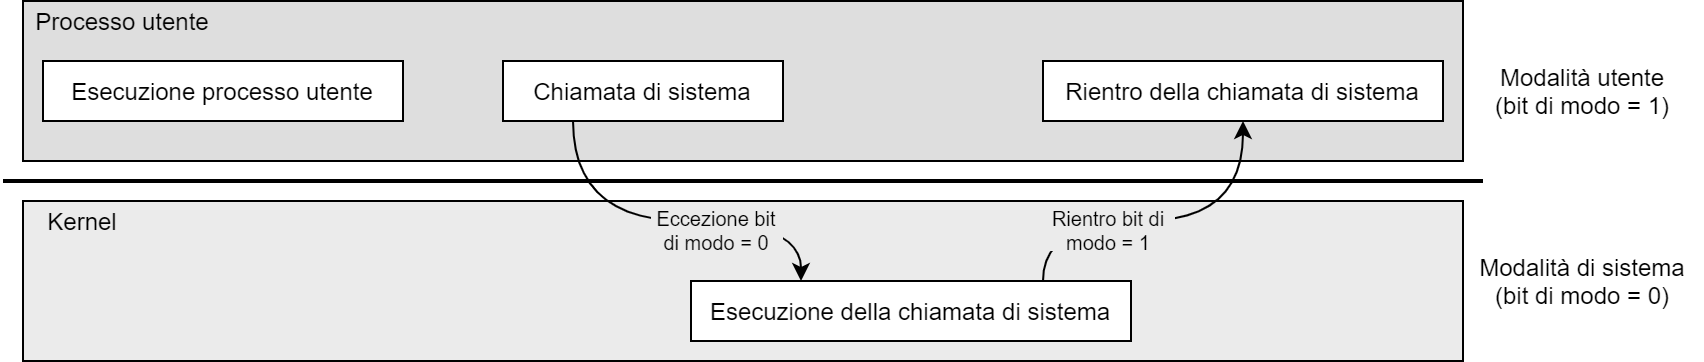
\includegraphics[width=1\textwidth]{img/img4.png}
            \caption{Transazione da modalità utente a modalità di sistema.}
            \label{fig:img4}
        \end{figure}
                
        Questa \textit{dual mode} garantisce anche la sicurezza del sistema nei confronti di operazioni dannose, in quanto vengono definite delle \textbf{istruzioni privilegiate} eseguibili solo in modalità di sistema, modalità a cui ovviamente l'utente non può fare accesso liberamente.
                
        Possono esserci anche più di due livelli, e infatti molti sistemi ne hanno di più.
                
    \subsection{Timer}
        Il \textbf{timer} è il modo che ha il sistema operativo per mantenere il controllo della CPU. Abbiamo un timer programmabile affinché invii un segnale d'interruzione a intervalli di tempo specificati, che possono essere fissi o variabili. Prima di restituire all'utente il controllo dell'esecuzione, il sistema operativo assegna un valore al timer. Allo scadere di questo valore genera un'interruzione che causa il trasferimento del controllo al sistema operativo, che potrà decidere se lasciare altro tempo al programma o interpretare l'interruzione come un errore fatale. Ovviamente, le istruzioni di controllo del timer sono eseguibili solo in modalità privilegiata.
                
\section{Gestione delle risorse}
    Come abbiamo già accennato il sistema operativo può essere visto come un gestore di risorse. Andiamo a vedere ora come gestisce tali risorse.
    
    \subsection{Gestione dei processi}
        Abbiamo già visto il concetto di processo. Un processo può eseguire una serie di compiti, ma per ora lo consideriamo come un lavoro d'elaborazione (\textit{job}) eseguito in un ambiente time-sharing, anche se il concetto è più generale.
        
        Il compito di gestire le risorse usate dei processi ce l'ha il sistema operativo, che può assegnarne alla creazione del processo o in maniera dinamica durante la sua esecuzione.
        
        C'è da specificare che un programma di per sé è un'entità passiva, mentre il processo è un'entità attiva. Un processo a singolo \textit{thread} ha un'esecuzione sequenziale; ha una serie di istruzioni che vengono eseguite una dopo l'altra. Un \textbf{contatore di programma} tiene il conto della prossima istruzione da eseguire, e anche se due processi appartengono allo stesso programma si considerano due sequenze di istruzioni separate. Un processo multithread ha più contatori di programma, ognuno dei quali punta all'istruzione da eseguire per il dato thread.
        
        Il processo è l'unità di lavoro di un sistema, e infatti il sistema può essere visto come un insieme di processi (alcuni eseguono codice del sistema, altri codice utente), che possono potenzialmente essere eseguiti in modo concorrente. Il sistema operativo ha la responsabilità di eseguire le seguenti attività connesse alla gestione dei processi:
        \begin{itemize}
            \item Creazione e cancellazione di processi utente e di sistema.
            \item Scheduling di processi e thread sulle CPU.
            \item Sospensione e ripristino dei processi.
            \item Fornitura di meccanismi per la sincronizzazione dei processi.
            \item Fornitura di meccanismi per la comunicazione fra processi.
        \end{itemize}
        
    \subsection{Gestione della memoria}
        La memoria centrale è un vasto vettore che può contenere fino a miliardi di parole, ognuna con il suo indirizzo. Generalmente è l'unico grande dispositivo di memorizzazione a cui la CPU può far riferimento e accedere in modo diretto.
        
        I sistemi moderni devono tenere in memoria molti programmi e dati, e la maniera in cui ottimizzano questo compito dipende dallo schema di gestione utilizzato, che può variare di efficacia in base a molti fattori, fra cui il tipo di architettura hardware del sistema.
        
        Il sistema operativo è responsabile di tenere traccia di quali parti di memoria sono attualmente in uso e da chi, di assegnare e revocare lo spazio di memoria secondo necessità, e infine di decidere quali processi (o parti di essi) e dati debbano essere caricati in memoria centrale o trasferiti nella memoria di massa.
        
    \subsection{Gestione dei file}
        Il sistema operativo definisce un'unità logica di archiviazione allo scopo di dare un'interfaccia chiara e uniforme, nella forma del \textbf{file}. Questo concetto è uno dei più visibili del sistema operativo, ma anche uno dei più generali; un file può avere vari formati, da molto liberi, ad eseguibili, a rigidamente formattati, come un file MP3.
        
        I file possono essere organizzati in directories per facilitarne la gestione, e inoltre se diversi utenti utilizzano il sistema potrebbe essere desiderabile controllare chi ha accesso a un determinato file.
        
        Il sistema operativo è responsabile delle seguenti attività connesse alla gestione dei file:
        \begin{itemize}
            \item Creazione e cancellazione dei file.
            \item Creazione e cancellazione delle directory.
            \item Fornire le funzioni fondamentali per la gestione di file e directory.
            \item Associazione di file a dispositivi di memoria secondaria.
            \item Creazione di backup di file su dispositivi di memoria non volatili.x
        \end{itemize}
        
    \subsection{Gestione della memoria di massa}
        La maggior parte dei sistemi operativi moderni usa memorie secondarie, spesso dischi magnetici o NVM, per immagazzinare dati e programmi (sono usati sia come sorgente che come destinazione dei dati creati). Il sistema operativo è responsabile delle seguenti attività connesse alla memoria di massa:
        \begin{itemize}
            \item Montare (\textit{mounting}) e smontare (\textit{unmounting}) le unità di memoria.
            \item Gestione dello spazio libero.
            \item Assegnazione dello spazio.
            \item Sceduling del disco.
            \item Partizionamento.
            \item Protezione.
        \end{itemize}
        
        La natura di questo tipo di memoria può variare in base all'uso che si intende farne. A volte potrebbe essere desiderabile un dispositivo più capiente ma più lento.
        
        Un altro tipo di memoria da citare è la \textbf{memoria terziaria}, composta da CD-ROM, chiavette USB, eccetera. Il sistema potrebbe decidere di gestire direttamente questi dispositivi come di delegarne la gestione a programmi applicativi.
        
    \subsection{Gestione della cache}
        Questo è un concetto importante di un sistema elaborativo. Solitamente le informazioni sono mantenute in memoria centrale, e al momento del loro utilizzo si copiano in un'unità più veloce, la \textbf{cache} appunto.
        
        Quando si deve utilizzare un'informazione si controlla se è presente nella cache e nel caso si usa quella copia, altrimenti si esegue una copia e la si mantiene in cache, sulla supposizione che presto servirà nuovamente.
        
        Data la limitata capacità della cache, la sua gestione è un importante problema di progettazione. Per esempio una questione molto delicata è quella delle multiple copia di un singolo oggetto; avendo vari tipi di memoria disposti in maniera gerarchica, un dato potrebbe essere in più di queste memorie contemporaneamente. Dobbiamo assicurarci, nel caso di un sistema multiprocessore, che venga presa la versione di questo dato aggiornata più di recente. La questione diventa ancora più delicata quando abbiamo più CPU, in quanto ogni CPU ha una sua cache locale, e i dati fra queste varie cache devono essere coerenti, dando vita appunto al problema della \textbf{coerenza della cache}, e che solitamente si risolve a livello di hardware, lasciando fuori quindi il sistema operativo. Andando a disperdere ancora di più i dati, quindi in sistemi distribuiti, la questione della coerenza diventa ancora più delicata, facendo sorgere la necessità di mantenere la coerenza del dato fra calcolatori diversi, i quali si trovano potenzialmente in locazioni geografiche disparate.
        
    \subsection{Gestione dell'I/O}
        Un compito del sistema operativo è quello di nascondere agli utenti le peculiarità dei vari dispositivi. In UNIX, per esempio, le caratteristiche dei dispositivi di I/O sono nascoste alla maggior parte dello stesso sistema operativo dal \textbf{sottosistema di I/O}, che è composto dalle seguenti parti:
        
        \begin{itemize}
            \item Un componente di gestione della memoria, fra cui gestione di buffer di I/O, gestione della cache e gestione delle aree di memoria per l'I/O asincrono (\textit{spooling}).
            \item Un'interfaccia generale per i driver dei dispositivi.
            \item I driver per gli specifici dispositivi.
        \end{itemize}
        
        Solo il driver del dispositivo conosce le peculiarità del dispositivo cui è assegnato.
        
\section{Virtualizzazione}
    La \textbf{virtualizzazione} è una tecnica che permette di astrarre l'hardware di un singolo computer (CPU, memoria, etc.) in diversi ambienti di esecuzione, creando così l'illusione che ogni distinto ambiente sia in esecuzione sul proprio computer. Un utente di una cosiddetta \textbf{macchina virtuale} può passare da un sistema operativo a un altro esattamente come in una situazione normale passa tra processi di esecuzione in un singolo sistema operativo.
    
    La virtualizzazione permette quindi a interi sistemi operativi di funzionare come fossero applicazioni all'interno di altri sistemi operativi. Questo fa parte di una tipologia di software che include l'\textbf{emulazione}, la quale tende a essere meno performante, soprattutto se le prestazioni della CPU emulatrice e quella emulata sono simili, in quanto ogni singola istruzione della CPU emulata deve essere replicata.
    
    Abbiamo due tipi di virtualizzazione:
    \begin{itemize}
        \item \textbf{Full virtualization:} Emula ogni cosa, fino alle istruzioni assembler.
        \item \textbf{Para-virtualization:} Prevede che ci sia una macchina in un dominio privilegiato \texttt{dom0} e tanti sistemi in altri domini che per eseguire proessi usano i servizi della macchina in \texttt{dom0}.
    \end{itemize}